\documentclass[11pt]{article}

\usepackage[margin=1in]{geometry}
\usepackage{amsmath, amssymb, amsthm}
\usepackage{tikz}
\usetikzlibrary{decorations.pathmorphing, arrows.meta, positioning, fit, backgrounds}
\usepackage{subcaption}
\usepackage{graphicx}
\usepackage{algorithm}
\usepackage{algorithmic}
\usepackage{hyperref}
\usepackage{natbib}
\usepackage{booktabs}

\newtheorem{definition}{Definition}
\newtheorem{theorem}{Theorem}
\newtheorem{corollary}{Corollary}
\newtheorem{lemma}{Lemma}
\newtheorem{proposition}{Proposition}
\newtheorem{example}{Example}

\title{Coarsening Causal Models with Cycles}
\author{
    Francisco Madaleno \\
    \textit{Department of Technology, Management and Economics,}\\
    \textit{Danish Technical University}
    \and
    Pratik Misra \\
    \textit{Department of Mathematics and Statistics,}\\
    \textit{Binghamton University, State University of New York}
    \and
    Alex Markham \\
    \textit{Department of Mathematical Sciences,}\\
    \textit{University of Copenhagen}
}
\date{}

\begin{document}
\maketitle

\begin{abstract}
Causal discovery in cyclic systems faces a fundamental obstacle: \citet{lacerda2008discovering} showed that a linear non-Gaussian cyclic structural equation model (SEM) is identifiable only up to a \emph{distributional equivalence class}, in which different graphs share the same observational distribution and are connected by reversals of cycles. We show that when the equivalence class is collapsed to the level of strongly connected components (SCCs), this ambiguity disappears: the \emph{condensation} (SCC partition together with inter-SCC edges) is invariant across the entire class and is therefore observationally identifiable. We obtain this result by combining the coarsening framework of \citet{madaleno2025coarsening} with the cyclic-SEM identification literature. The coarsening lattice acquires a structural floor — nodes in the same SCC must lie in the same block of any valid DAG-coarsening — and the SCC partition is the finest valid coarsening; its quotient graph is the condensation. Under linear non-Gaussian SEMs with no latent confounders, the support of the (square) ICA mixing matrix is the transitive closure of $G$, whose SCC partition equals that of $G$, so a single Tarjan pass on $\operatorname{supp}(\hat A)$ recovers the floor. Inter-SCC edges follow from $\hat B = I - \hat A^{-1}$ as in \citet{lacerda2008discovering}. Under soft interventions \texttt{RePaRe} requires no modification, since nodes within an SCC share intervened-ancestor signatures. Synthetic experiments confirm the theorem: inter-SCC edge $F_1$ converges to one with sample size while variable-level $F_1$ saturates strictly below one, the gap being the unidentifiable intra-SCC structure. Because the condensation is a DAG, cluster-level causal effects are identifiable on it via existing C-DAG identification machinery \citep{anand2023causal}, providing a downstream payoff for the recovered structure.
\end{abstract}


% =============================================================================
\section{Introduction}
% =============================================================================

Causal discovery from observational data has predominantly focused on directed \emph{acyclic} graphs (DAGs). Yet many systems of scientific interest contain feedback loops: gene-regulatory networks, ecological food webs, economic equilibria, and engineered control systems all exhibit directed cycles. A separate line of work on \emph{cyclic} causal models has therefore developed, ranging from the structural-equation formulation of \citet{spirtes1995directed,bongers2021foundations} to the linear non-Gaussian models of \citet{lacerda2008discovering}, which exploit standard ICA \citep{eriksson2004identifiability} to identify the mixing matrix $A = (I - B)^{-1}$ of a linear cyclic SEM up to column permutation and scaling, from which the cyclic graph $G$ can in principle be recovered.

In a separate development, the \emph{coarsening} framework of \citet{madaleno2025coarsening} addresses a different brittleness in the standard pipeline: many tasks do not require a fine-grained graph but rather an abstraction that pools indistinguishable variables. Given a fine-grained DAG $G$ and a set of interventions $\mathcal{I}$, the interventional coarsening $G^{\mathcal{I}}$ groups variables that share intervened-ancestor signatures, and the \texttt{RePaRe} algorithm provably recovers this coarsening from data. The framework is acyclic throughout, however: every coarsening it considers is a DAG and the underlying graph is required to be one as well.

\paragraph{Contributions.} We extend the coarsening framework to directed graphs that may contain cycles, and connect it to the cyclic-SEM identification literature. Concretely:
\begin{itemize}
    \item \textbf{Condensation identifiability (Theorem~\ref{thm:condensation-id}, \S\ref{sec:approach-oica}).} The condensation DAG of a linear non-Gaussian cyclic SEM is invariant across Lacerda's distributional equivalence class. The cluster DAG is therefore identifiable from observational data alone, without invoking the stability + disjoint-cycles assumption of \citet{lacerda2008discovering}.
    \item \textbf{The SCC floor (\S\ref{sec:scc-floor}).} The coarsening lattice acquires a structural floor: any valid DAG-coarsening must group nodes in a common SCC, and the SCC partition is the finest valid coarsening. This is the structural reason why condensation identifiability holds.
    \item \textbf{Intervention-determined recovery (\S\ref{sec:approach-ivn}).} Under soft (shift) interventions on a linear cyclic SEM, nodes in the same SCC share identical intervened-ancestor signatures, so \texttt{RePaRe} recovers the SCC floor without modification.
    \item \textbf{Causal-effect identification on the condensation (\S\ref{sec:effects}).} Since the condensation is acyclic, the C-DAG identification theorems of \citet{anand2023causal} apply directly: cluster-level effects are identifiable from the recovered structure.
    \item \textbf{Empirical verification (\S\ref{sec:experiments}).} On synthetic linear cyclic SEMs the \texttt{Lacerda} recipe attains inter-SCC edge $F_1 \to 1$ with sample size, while variable-level $F_1$ saturates strictly below one — the gap reflects the unidentifiable intra-SCC structure, by design.
\end{itemize}

The paper is organised as follows: \S\ref{sec:background} fixes notation and recalls the coarsening lattice and cyclic-SEM background; \S\ref{sec:cycles} introduces DAG-coarsenings of cyclic graphs, proves the SCC-floor proposition, presents the two recovery procedures, and proves condensation identifiability; \S\ref{sec:effects} discusses the implication for cluster-level causal-effect identification; \S\ref{sec:experiments} reports the synthetic experiments; \S\ref{sec:discussion} concludes. All proofs are in the appendix.


% =============================================================================
\section{Related Work}
\label{sec:related}
% =============================================================================

\paragraph{Cyclic causal models.} Cyclic generalisations of structural causal models date back to \citet{spirtes1995directed}, with rigorous foundations in \citet{bongers2021foundations}. \citet{lacerda2008discovering} showed that linear non-Gaussian cyclic SEMs with no latent confounders can be identified via standard ICA, by computing $\hat B = I - \hat A^{-1}$ and thresholding. Later work has extended this to latent-confounded settings via overcomplete ICA \citep{salehkaleybar2020learning, dai2026distributional}, group-wise extensions of LiNGAM \citep{maeda2020rcd}, and constraint-based methods using $\sigma$-separation \citep{forre2018constraint}.

\paragraph{Coarsening and abstraction of causal models.} Coarsening of causal models has been approached from several angles: causal abstraction in the structural-causal-model sense \citep{rubenstein2017causal,beckers2020approximate}, group-level structure under partial-order assumptions \citep{wahl2025foundations}, the structural-baseline coarsening of \citet{petersen2025structural}, and the partition-refinement approach of \citet{madaleno2025coarsening} that we extend here. Once a cluster-level causal graph (C-DAG) is in hand, the identification theorems of \citet{anand2023causal} characterise which cluster-level interventional distributions are recoverable from observational data, providing the natural downstream consumer of our identification result.

\paragraph{Relation to \citet{dai2026distributional}.} Our argument uses a single ingredient from \citet{dai2026distributional}, namely the path-rank lemma stating that $\operatorname{supp}(A) = \operatorname{adjacency}(G^{*})$ for $A = (I - B)^{-1}$ generically. \citet{dai2026distributional} are concerned with the latent-confounded setting and use overcomplete ICA; we work in the no-latent-confounders regime where standard square ICA suffices, and the central condensation-identifiability result (Theorem~\ref{thm:condensation-id}) is established here independently from their characterisation of distributional equivalence.

\paragraph{Strongly connected components and condensation.} The condensation construction is standard in graph theory; \citet{tarjan1972depth} gives a linear-time algorithm and \citet{gabow2000path} a path-based alternative. Our use of the SCC partition as the finest valid DAG-coarsening is, to our knowledge, new in the causal-discovery context, though closely related observations underlie the ICA-based identifiability results cited above.


% =============================================================================
\section{Background}
\label{sec:background}
% =============================================================================

We recall the key definitions from~\citet{madaleno2025coarsening}. A \emph{coarsening} of a DAG $G = (V, E)$ is a DAG $G' = (V', E')$ together with a surjection $\chi: V \to V'$ such that $E' = \{\chi(v) \to \chi(w) \mid v \to w \in E, \chi(v) \neq \chi(w)\}$. Equivalently, a coarsening is a partition $\Pi = \{\pi_1, \ldots, \pi_k\}$ of $V$ whose induced quotient graph is a DAG.

The set of all coarsenings of $G$, ordered by refinement, forms a sublattice of the partition refinement lattice (Theorem~3 in~\citet{madaleno2025coarsening}). The \texttt{RePaRe} algorithm traverses this lattice using two oracles: \texttt{Refine} splits a block of the partition, and \texttt{IsEdge} determines adjacency between blocks.

\subsection{Cyclic structural equation models}

A linear cyclic SEM (also called structural equations with cycles, SEwC) is defined by:
\begin{equation}\label{eq:sem}
    X = BX + E, \qquad \text{solved as } X = (I - B)^{-1} E,
\end{equation}
where $B \in \mathbb{R}^{d \times d}$ is the weighted adjacency matrix of a directed graph $G$ (which may contain cycles) and $E$ has mutually independent components. The solution exists and is unique when the spectral radius $\rho(B) < 1$.

Under a soft (shift) intervention on node $k$:
\begin{equation}\label{eq:soft}
    X^{I} = (I - B)^{-1}(E + \delta_k e_k),
\end{equation}
so intervention effects propagate through the entire graph, including back through cycles. Hard (do) interventions, which set $X_k = c$ by severing the equation for node $k$, are excluded: they break the cyclic mechanism and can render the system inconsistent.


% =============================================================================
\section{Coarsening Directed Graphs with Cycles}
\label{sec:cycles}
% =============================================================================

We first generalise the notion of coarsening from DAGs to directed graphs that may contain cycles.

\begin{definition}[DAG coarsening of a directed graph]\label{def:dag-coarsening}
    Given a directed graph $G = (V, E)$ which may contain cycles, a \emph{DAG coarsening} of $G$ is a partition $\Pi$ of $V$ together with a surjective mapping $\chi : V \to V'$ assigning each node to its block, such that the quotient graph $G' = (V', E')$ defined by
    \[
        E' = \{(\chi(u), \chi(v)) \mid (u, v) \in E,\ \chi(u) \neq \chi(v)\}
    \]
    is acyclic.
\end{definition}

When $G$ is a DAG this reduces to the original definition of~\citet{madaleno2025coarsening}: the trivial single-block-per-node partition has an acyclic quotient, and so does any coarsening of it. For general directed graphs the acyclicity requirement is non-trivial and forces SCCs to be respected, as Proposition~\ref{prop:scc-floor} below shows.

\subsection{The SCC floor}
\label{sec:scc-floor}

Condition~1 of Definition~\ref{def:dag-coarsening} imposes a structural floor on the coarsening lattice.

\begin{proposition}[SCC floor]\label{prop:scc-floor}
    Let $G = (V, E)$ be a directed graph. Nodes $v, w \in V$ that belong to the same strongly connected component of $G$ must be in the same block of any valid coarsening. Consequently, the SCC partition is the finest valid DAG-coarsening of $G$.
\end{proposition}

\begin{proof}
    If $v$ and $w$ are in the same SCC, there exist directed paths $v \to \cdots \to w$ and $w \to \cdots \to v$ in $G$. If $\chi(v) \neq \chi(w)$ in a coarsening, these paths induce directed paths $\chi(v) \to \cdots \to \chi(w)$ and $\chi(w) \to \cdots \to \chi(v)$ in the coarsened graph, forming a cycle and violating the DAG requirement.
\end{proof}

The SCC partition is computable in $O(|V| + |E|)$ via Tarjan's algorithm~\citep{tarjan1972depth}; for graphs with many SCCs Gabow's path-based algorithm can be modestly faster in practice~\citep{gabow2000path}.

\paragraph{Remark: cyclic coarsenings.}
Definition~\ref{def:dag-coarsening} requires the coarsened graph to be a DAG, mirroring the original framework of \citet{madaleno2025coarsening}. A natural generalisation drops this requirement and asks only that the coarsening preserves the partial order over SCCs of $G$: any partition $\chi$ such that the quotient graph (a) does not reverse a non-cyclic ancestral relation in $G$, and (b) does not introduce a cycle between nodes that are not already in a common SCC, is a valid \emph{cyclic coarsening}. The interventional and observational coarsenings considered below are all valid DAG-coarsenings (and hence cyclic coarsenings), so we focus on the DAG case throughout. The general cyclic-coarsening lattice is interesting in its own right and we leave its characterisation to future work.

\begin{example}[Illustrative coarsening]\label{ex:illustrative}
Consider a system with eight variables $V = \{a, b, c, d, e, f, g, h\}$ whose micro-level interactions contain feedback loops (Figure~\ref{fig:example}a):
\begin{itemize}
    \item $a, b, e$ form a directed 3-cycle ($a \to b \to e \to a$).
    \item $c, d, h$ form an SCC via interlocking 2-cycles ($c \leftrightarrow d$ and $d \leftrightarrow h$).
    \item $f, g$ form a directed 2-cycle ($f \leftrightarrow g$).
    \item Cross-component edges: $b \to c$, $b \to f$, $e \to f$, $c \to g$, $h \to g$.
\end{itemize}
Since any DAG coarsening must absorb each SCC into a single macro-node (Definition~\ref{def:dag-coarsening}), the finest valid coarsening maps $\chi: V \to \{A', C', F'\}$ with $A' = \{a,b,e\}$, $C' = \{c,d,h\}$, $F' = \{f,g\}$, yielding the condensation DAG in Figure~\ref{fig:example}b.
\end{example}

\begin{figure}[t]
    \centering
    \begin{subfigure}[b]{0.62\textwidth}
        \centering
        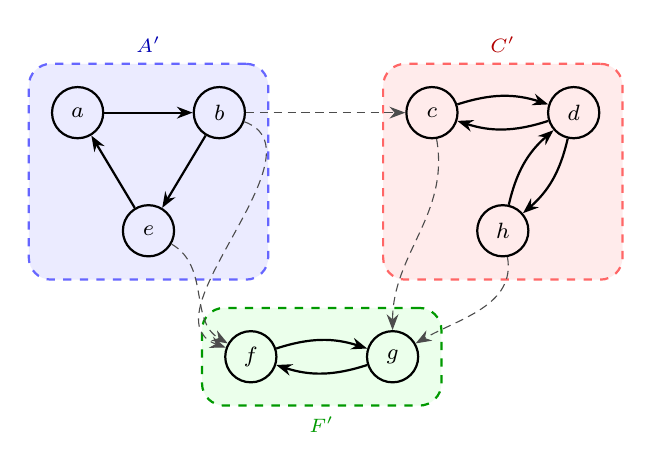
\begin{tikzpicture}[
            vertex/.style={circle, draw, thick, minimum size=6.5mm, inner sep=0pt, font=\footnotesize\bfseries},
            intra/.style={-{Stealth[length=2mm]}, thick},
            cross/.style={-{Stealth[length=2mm]}, gray!60!black, densely dashed},
            sccbox/.style={rounded corners=8pt, dashed, thick, inner sep=8pt}
        ]
            % SCC1: {a, b, e}
            \node[vertex] (a) at (0, 1.8) {$a$};
            \node[vertex] (b) at (1.8, 1.8) {$b$};
            \node[vertex] (e) at (0.9, 0.3) {$e$};

            % SCC2: {c, d, h}
            \node[vertex] (c) at (4.5, 1.8) {$c$};
            \node[vertex] (d) at (6.3, 1.8) {$d$};
            \node[vertex] (h) at (5.4, 0.3) {$h$};

            % SCC3: {f, g}
            \node[vertex] (f) at (2.2, -1.3) {$f$};
            \node[vertex] (g) at (4.0, -1.3) {$g$};

            % SCC backgrounds
            \begin{scope}[on background layer]
                \node[sccbox, draw=blue!60, fill=blue!8,
                      fit=(a)(b)(e),
                      label={[font=\scriptsize\sffamily, blue!70!black]above:$A'$}] {};
                \node[sccbox, draw=red!60, fill=red!8,
                      fit=(c)(d)(h),
                      label={[font=\scriptsize\sffamily, red!70!black]above:$C'$}] {};
                \node[sccbox, draw=green!60!black, fill=green!8,
                      fit=(f)(g),
                      label={[font=\scriptsize\sffamily, green!60!black]below:$F'$}] {};
            \end{scope}

            % Intra-SCC1 edges (3-cycle)
            \draw[intra] (a) -- (b);
            \draw[intra] (b) -- (e);
            \draw[intra] (e) -- (a);

            % Intra-SCC2 edges (interlocking 2-cycles)
            \draw[intra, bend left=18] (c) to (d);
            \draw[intra, bend left=18] (d) to (c);
            \draw[intra, bend left=18] (d) to (h);
            \draw[intra, bend left=18] (h) to (d);

            % Intra-SCC3 edges (2-cycle)
            \draw[intra, bend left=18] (f) to (g);
            \draw[intra, bend left=18] (g) to (f);

            % Cross-SCC edges
            \draw[cross] (b) -- (c);
            \draw[cross] (b) to[out=-20, in=160] (f);
            \draw[cross] (e) to[out=-30, in=150] (f);
            \draw[cross] (c) to[out=-80, in=90] (g);
            \draw[cross] (h) to[out=-80, in=30] (g);
        \end{tikzpicture}
        \caption{Micro-level directed graph $G$ with three SCCs (shaded regions). Solid arrows are intra-SCC edges; dashed arrows are cross-component edges.}
        \label{fig:example-micro}
    \end{subfigure}
    \hfill
    \begin{subfigure}[b]{0.32\textwidth}
        \centering
        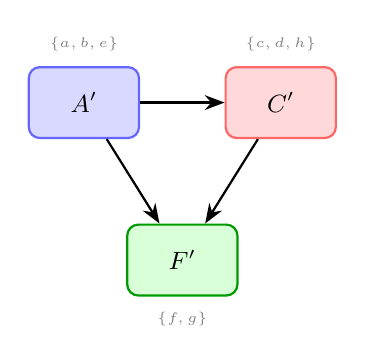
\begin{tikzpicture}[
            macro/.style={rectangle, rounded corners=4pt, draw, thick,
                          minimum width=14mm, minimum height=9mm,
                          font=\small\sffamily\bfseries},
            edge/.style={-{Stealth[length=2.5mm]}, thick}
        ]
            \node[macro, fill=blue!15, draw=blue!60] (A) at (0, 2.5) {$A'$};
            \node[macro, fill=red!15, draw=red!60] (C) at (2.5, 2.5) {$C'$};
            \node[macro, fill=green!15, draw=green!60!black] (F) at (1.25, 0.5) {$F'$};

            \draw[edge] (A) -- (C);
            \draw[edge] (A) -- (F);
            \draw[edge] (C) -- (F);

            \node[font=\tiny\sffamily, text=gray, above=2pt] at (A.north) {$\{a,b,e\}$};
            \node[font=\tiny\sffamily, text=gray, above=2pt] at (C.north) {$\{c,d,h\}$};
            \node[font=\tiny\sffamily, text=gray, below=2pt] at (F.south) {$\{f,g\}$};
        \end{tikzpicture}
        \caption{Condensation DAG $G'$: the finest valid DAG coarsening.}
        \label{fig:example-condensation}
    \end{subfigure}
    \caption{A cyclic micro-level directed graph (a) and its coarsened macro-level DAG (b), for the system in Example~\ref{ex:illustrative}. Each SCC is contracted to a single macro-node; cross-component edges induce the edges of the condensation.}
    \label{fig:example}
\end{figure}

\paragraph{Combinatorial structure of the lattice.}
The full partition lattice of $n$ nodes is organised by block count~$k$, with the number of $k$-block partitions given by the Stirling numbers of the second kind $S(n, k)$, computed via the recurrence $S(n,k) = k \cdot S(n-1,k) + S(n-1,k-1)$. For $n = 8$:
\[
    S(8,1) = 1, \; S(8,2) = 127, \; S(8,3) = 966, \; S(8,4) = 1701, \; S(8,5) = 1050, \; S(8,6) = 266, \; S(8,7) = 28, \; S(8,8) = 1,
\]
yielding a Bell number of $B_8 = \sum_{k=1}^{8} S(8,k) = 4{,}140$ total partitions. For the graph of Example~\ref{ex:illustrative}, only 4 of these are valid DAG coarsenings --- one trivial single-block partition, two at the 2-block level, and the SCC floor at $k = 3$. Every partition finer than the SCC floor necessarily splits at least one strongly connected component, producing a cycle in the quotient graph. Figure~\ref{fig:lattice} visualises this structure.

\begin{figure}[t]
    \centering
    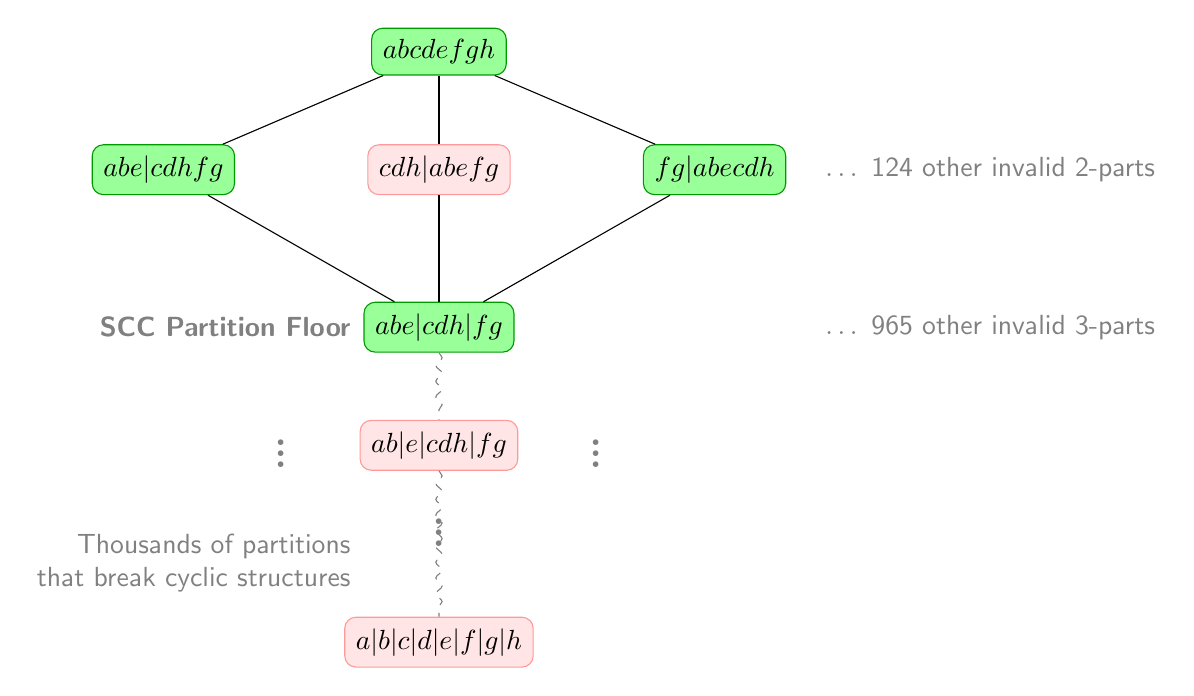
\begin{tikzpicture}[
        node distance=1.5cm and 2.5cm,
        valid/.style={rectangle, rounded corners, fill=green!40!white, inner sep=4pt, font=\sffamily, draw=green!60!black},
        invalid/.style={rectangle, inner sep=4pt, font=\sffamily, text=gray},
        invalidbox/.style={rectangle, rounded corners, fill=red!10!white, inner sep=4pt, font=\sffamily, draw=red!40!white},
        dots/.style={font=\Huge, text=gray}
    ]

    % Level 0: 1 part (Top)
    \node[valid] (top) at (0, 0) {$abcdefgh$};

    % Level 1: 2 parts (Macro level)
    \node[valid] (A_CF) at (-3.5, -1.5) {$abe | cdhfg$};
    \node[invalidbox] (C_AF) at (0, -1.5) {$cdh | abefg$}; % Invalid due to induced cycle
    \node[valid] (F_AC) at (3.5, -1.5) {$fg | abecdh$};
    \node[invalid] (other_2) at (7, -1.5) {$\dots$ 124 other invalid 2-parts};

    % Level 2: 3 parts (The SCC Floor)
    \node[valid] (bottom_valid) at (0, -3.5) {$abe | cdh | fg$};
    \node[invalid] (other_3) at (7, -3.5) {$\dots$ 965 other invalid 3-parts};

    % Level 3-6: The vast invalid space (Splitting SCCs)
    \node[dots] (d1) at (-2, -5) {$\vdots$};
    \node[invalidbox] (split_ex1) at (0, -5) {$ab | e | cdh | fg$}; % Example of a split cycle
    \node[dots] (d2) at (2, -5) {$\vdots$};

    \node[dots] (d3) at (0, -6) {$\vdots$};

    % Level 7: 8 parts (The Absolute Bottom)
    \node[invalidbox] (absolute_bottom) at (0, -7.5) {$a | b | c | d | e | f | g | h$};

    % --- Edges ---
    % Valid macro edges
    \draw (top) -- (A_CF);
    \draw (top) -- (C_AF);
    \draw (top) -- (F_AC);

    \draw (A_CF) -- (bottom_valid);
    \draw (C_AF) -- (bottom_valid);
    \draw (F_AC) -- (bottom_valid);

    % Paths into the invalid abyss
    \draw[gray, dashed, decorate, decoration={snake, amplitude=.4mm, segment length=2mm, post length=1mm}] (bottom_valid) -- (split_ex1);
    \draw[gray, dashed, decorate, decoration={snake, amplitude=.4mm, segment length=2mm, post length=1mm}] (split_ex1) -- (absolute_bottom);

    % Annotations
    \node[anchor=east, font=\sffamily\bfseries\color{gray}] at (-1, -3.5) {SCC Partition Floor};
    \node[anchor=east, font=\sffamily\color{gray}, align=right] at (-1, -6.5) {Thousands of partitions\\that break cyclic structures};

    \end{tikzpicture}
    \caption{The valid DAG-coarsening sublattice (green) embedded in the full partition lattice ($B_8 = 4{,}140$ partitions) for the graph of Example~\ref{ex:illustrative}. Only 4 of the 4{,}140 partitions are valid: the single-block top, two 2-block coarsenings that respect all SCCs, and the SCC floor $\{abe \mid cdh \mid fg\}$. Red nodes show invalid partitions that split at least one SCC, inducing a cycle in the quotient graph.}
    \label{fig:lattice}
\end{figure}


\subsection{Approach 1: Intervention-determined coarsening}
\label{sec:approach-ivn}

Under soft interventions, the cyclic SEM becomes $X^{I} = (I-B)^{-1}(E + \delta)$, so intervention effects propagate through the entire graph, including back through cycles. Nodes within the same SCC are mutual ancestors and therefore share identical intervened-ancestor signatures: $\mathcal{I}\text{-an}_G(v) = \mathcal{I}\text{-an}_G(w)$ for all $v, w$ in the same SCC. Consequently, \texttt{RefineTest} can never split an SCC, and \texttt{RePaRe} recovers the interventional coarsening $G^{\mathcal{I}}$ with the SCC partition as its floor --- without any modification to the algorithm.


\subsection{Approach 2: Observational coarsening via linear non-Gaussian ICA}
\label{sec:approach-oica}

We assume the linear cyclic SEM of \eqref{eq:sem} with mutually independent, non-Gaussian noise terms $E_i$ and \emph{no latent confounders}, so the noise vector $E$ has the same dimension as $X$. Under these assumptions the mixing matrix $A = (I-B)^{-1}$ is square, full-rank (since $\rho(B) < 1$), and identifiable from the distribution of $X = AE$ up to column permutation and scaling \citep{eriksson2004identifiability}, via standard (non-overcomplete) ICA. This is the regime exploited by \citet{lacerda2008discovering} for cyclic causal discovery; overcomplete ICA \citep{lewicki2000learning} is needed only when the number of independent sources exceeds the number of observed variables, which arises with latent confounders \citep{salehkaleybar2020learning, dai2026distributional}.

\paragraph{The mixing matrix encodes reachability.}
Expanding the Neumann series $A = I + B + B^2 + \ldots$, the entry $A_{ij}$ is the total causal effect of source $j$ on variable $i$, summed over all directed paths. Generically (i.e.\ for almost all parameterisations of $B$), $A_{ij} \neq 0$ if and only if there is a directed path from $j$ to $i$ in $G$ \citep{dai2026distributional}. Therefore $\operatorname{supp}(A)$ is the adjacency matrix of the transitive closure $G^*$ of $G$.

\paragraph{Transitive closure preserves SCCs.}
Adding transitive edges cannot create new mutual reachability nor destroy existing mutual reachability, so $\operatorname{SCC}(G^*) = \operatorname{SCC}(G)$ (Theorem~\ref{thm:scc-tc}, Appendix~\ref{app:proofs}). Running Tarjan's algorithm on $\operatorname{supp}(\hat A)$ thus recovers the SCC partition of $G$, even though we never observe $G$ directly.

\paragraph{From distributional equivalence class to identifiable C-DAG.}
\citet{lacerda2008discovering} showed that linear non-Gaussian cyclic SEMs are observationally identifiable only up to a distributional equivalence class, whose members differ by reversals of cycles in $G$ (Lacerda's Theorem~4). In particular the orientation of any single cycle is generally unrecoverable. The next theorem shows that this ambiguity vanishes once the equivalence class is collapsed to the level of strongly connected components.

\begin{theorem}[Condensation identifiability]\label{thm:condensation-id}
    Let $G_1, G_2$ be two directed graphs underlying linear cyclic SEMs of the form~\eqref{eq:sem}, both with no latent confounders, $\rho(B_i) < 1$, mutually independent noise terms and at most one Gaussian noise component. If they induce the same observational distribution over $X$, then their condensations are equal: same SCC partition, same set of inter-SCC edges.
\end{theorem}

\begin{proof}
    Equality of distributions implies that the mixing matrices $A_1 = (I - B_1)^{-1}$ and $A_2 = (I - B_2)^{-1}$ coincide up to column permutation and scaling \citep{eriksson2004identifiability,lacerda2008discovering}. The support of a matrix is invariant under column permutation and rescaling of nonzero columns, so $\operatorname{supp}(A_1) = \operatorname{supp}(A_2)$. By the path-rank identity \citep[Lemma~2]{dai2026distributional}, $\operatorname{supp}(A_i)$ is the adjacency of the transitive closure $G_i^{*}$. Hence $G_1^{*} = G_2^{*}$, and Theorem~\ref{thm:scc-tc} gives $\operatorname{SCC}(G_1) = \operatorname{SCC}(G_1^{*}) = \operatorname{SCC}(G_2^{*}) = \operatorname{SCC}(G_2)$, so the two SCC partitions agree.

    For the inter-SCC edges, recall that members of Lacerda's distributional equivalence class differ by reversals of cycles in $G$ (Lacerda's Theorem~4), and every such cycle is contained in a single SCC. Reversing a cycle modifies only intra-SCC entries of $B$ and leaves all inter-SCC entries unchanged. Hence the set of inter-SCC edges of $G_1$ and $G_2$ coincides as well, and the two condensations are equal.
\end{proof}

\begin{corollary}\label{cor:condensation-id}
    In the large-sample limit, the condensation of $G$ is recoverable by computing FastICA + Tarjan on $\operatorname{supp}(\hat A)$ and reading inter-SCC edges off $\hat B = I - \hat A^{-1}$, without invoking the stability assumption of \citet{lacerda2008discovering}.
\end{corollary}

\paragraph{Faithfulness on the condensation.}
A second consequence of the SCC aggregation is the validity of conditional-independence tests at the cluster level.

\begin{lemma}[Faithfulness on the condensation]\label{lem:cond-faith}
    Under the linear cyclic SEM of~\eqref{eq:sem} with $\sigma$-faithfulness, the marginal joint distribution on SCC-block features is Markov and faithful to the condensation DAG $G/\!\!\sim$.
\end{lemma}

\noindent
The argument is standard: linear cyclic SEMs are $\sigma$-Markov to $G$ \citep{spirtes1995directed,bongers2021foundations}, $\sigma$-separation collapses to ordinary d-separation when the graph is acyclic, and aggregating variables to SCC blocks projects $\sigma$-separation statements about $G$ onto d-separation statements about the (acyclic) condensation. Under $\sigma$-faithfulness, no cancellations introduce extra independencies, so the projected distribution is Markov \emph{and} faithful to $G/\!\!\sim$. In particular the same CI argument that justifies \texttt{IsEdge} in the original \texttt{RePaRe} carries over to inter-block features unchanged.

\paragraph{Algorithm.} This yields a procedure requiring only observational data — the \texttt{Lacerda} recipe, viewed through the coarsening lattice:
\begin{enumerate}
    \item \textbf{Estimate} $\hat A$ via FastICA \citep{hyvarinen1999fast}, with as many components as variables. Resolve the permutation ambiguity by maximising $\sum_i |\hat A_{i,\sigma(i)}|$ via the Hungarian algorithm \citep{kuhn1955hungarian}, exploiting $A_{ii} = 1$ from the identity term in the Neumann series. Normalise each column so that $\hat A_{ii} = 1$.
    \item \textbf{Compute} $\hat B = I - \hat A^{-1}$ and threshold its entries at $\tau$.
    \item \textbf{Recover the partition} $\hat\Pi$ as the SCCs of $\operatorname{supp}(\hat B)$ via Tarjan's algorithm \citep{tarjan1972depth}, and \textbf{recover the condensation edges} as the inter-block entries of $\operatorname{supp}(\hat B)$.
\end{enumerate}
Theorem~\ref{thm:condensation-id} guarantees that this procedure targets the correct object — the condensation of any data-generating graph in the distributional equivalence class — and Corollary~\ref{cor:condensation-id} guarantees consistency in the large-sample limit. An equivalent partition step uses $\operatorname{supp}(\hat A)$ directly, which avoids the $\kappa(\hat A)$-fold noise amplification incurred by inverting $\hat A$; the two thresholdings agree asymptotically.

\paragraph{Conservative behaviour at the partition step.} Estimation noise can cause entries of $\hat A$ to fall below $\tau$ and \emph{merge} distinct SCCs into a single block, but it can never \emph{split} a true SCC: a coarser-than-necessary partition is still a valid DAG-coarsening, whereas splitting an SCC would induce a cycle in the quotient graph and violate the DAG requirement.


% =============================================================================
\section{Causal Effect Identification on the Condensation}
\label{sec:effects}
% =============================================================================

Theorem~\ref{thm:condensation-id} elevates the recovered structure from a partition into a fully oriented C-DAG over clusters. Because the condensation is acyclic, the standard machinery of cluster-level causal-effect identification applies.

\paragraph{Cluster-level interventions in cyclic SEMs.} Hard interventions on a single variable break the cyclic mechanism (\S\ref{sec:background}) and are excluded throughout the paper. In contrast, a hard intervention on an \emph{entire SCC} simultaneously is well-defined: replacing all equations within a block $\pi$ with constants yields $X^{\,\mathrm{do}(\pi = c)} = (I_{V \setminus \pi} - B_{V \setminus \pi})^{-1} (E_{V \setminus \pi} + B_{V \setminus \pi,\,\pi}\, c)$, and the surrounding cyclic substructure outside $\pi$ remains consistent under $\rho(B) < 1$. Soft (shift) interventions on cluster members are likewise well-defined and, applied uniformly across $\pi$, induce a cluster-level shift on the C-DAG.

\paragraph{C-DAG identification.} Once the condensation $G/\!\!\sim$ is in hand, the C-DAG identification theorems of \citet{anand2023causal} apply directly: for clusters $C, Y$ in $G/\!\!\sim$, the cluster-level interventional distribution $P(Y \mid \mathrm{do}(C = c))$ is identifiable from $P(X)$ whenever the standard ID conditions hold on $G/\!\!\sim$. We do not introduce a new ID algorithm; the contribution is to observe that the condensation is the natural object on which existing C-DAG ID machinery operates, and that Theorem~\ref{thm:condensation-id} supplies its prerequisite from purely observational data, even though the underlying micro-graph $G$ is itself not identifiable.


% =============================================================================
\section{Experimental Results}
\label{sec:experiments}
% =============================================================================

We illustrate Theorem~\ref{thm:condensation-id} on synthetic linear non-Gaussian cyclic SEMs using the \texttt{Lacerda} recipe of \S\ref{sec:approach-oica}. The intervention-determined approach (\S\ref{sec:approach-ivn}) is theoretically covered by the unmodified guarantees of \citet{madaleno2025coarsening} and is not exercised here.

\subsection{Setup}

\paragraph{Data-generating process.} We generate linear non-Gaussian cyclic SEMs on $d = 10$ variables with a controlled number $\kappa \in \{3, 4, 5\}$ of non-trivial SCCs and edge densities $\rho \in \{0.3, 0.5, 0.8\}$. For each $(d, \kappa, \rho)$, the $d$ nodes are randomly partitioned into $\kappa$ non-trivial SCCs (each of size $\geq 2$) plus singleton nodes. Within each SCC a directed Hamilton cycle ensures mutual reachability and additional intra-SCC directed edges are sampled at probability $\rho$. Between blocks, edges that respect a random topological order over blocks are sampled at probability $\rho$. Edge weights are sampled in $[0.25, 0.75]$ with random sign and rescaled to enforce $\rho(B) < 1$. Noise terms $E_i$ are mutually independent and Laplace-distributed. Sample sizes range over $n \in \{50, 100, 500, 1000\}$; each cell is replicated across 3 random seeds.

\paragraph{Method.} We run a single observational pipeline, \texttt{Lacerda} \citep{lacerda2008discovering}: estimate $\hat A$ by FastICA with $d$ components, resolve the column-permutation ambiguity by the Hungarian algorithm and normalise each column so that $\hat A_{ii} = 1$, compute $\hat B = I - \hat A^{-1}$, threshold $|\hat B|$ at $\tau = 0.1$, and read both the SCC partition (Tarjan on $\operatorname{supp}(\hat B)$) and the inter-block edges off $\operatorname{supp}(\hat B)$. By Corollary~\ref{cor:condensation-id} this is consistent for the condensation in the large-sample limit.

\paragraph{Metrics.} Ground truth is the true SCC partition of $G$ (Tarjan on the data-generating $B$) and the corresponding condensation. We report:
\begin{itemize}
    \item \emph{ARI} of the predicted partition versus the true SCC partition;
    \item \emph{inter-SCC $F_1$}: $F_1$ of predicted variable-level edges, restricted to pairs $(i,j)$ in different true SCCs — the identifiable portion under our assumptions, the target of Theorem~\ref{thm:condensation-id};
    \item \emph{variable-level $F_1$}: $F_1$ over all directed edges (including intra-SCC), to quantify the gap between identifiable and unidentifiable structure.
\end{itemize}

\subsection{Results}

Figure~\ref{fig:results} shows partition and edge recovery as functions of sample size, faceted by $\kappa$. Three observations:
\begin{itemize}
    \item \emph{Partition recovery (ARI).} ARI rises with $n$ and approaches 1, confirming consistency of FastICA + Tarjan under non-Gaussian noise and $\rho(B) < 1$. Below $n \approx 500$ partitions are unstable.
    \item \emph{Inter-SCC edges.} Inter-SCC $F_1$ converges to 1 with $n$, directly illustrating Theorem~\ref{thm:condensation-id}: the inter-SCC structure is identifiable, and \texttt{Lacerda} attains it asymptotically.
    \item \emph{Variable-level $F_1$.} Variable-level $F_1$ saturates strictly below 1 even at the largest sample sizes. The gap is the unidentifiable intra-SCC mass: in expectation the maximum attainable variable-level $F_1$ from \emph{any} observational method is the inter-SCC fraction of the total edge set, since intra-SCC edge orientations are interchangeable across the distributional equivalence class. The gap is therefore not a defect of the method but a property of the identification target.
\end{itemize}
This is precisely the picture predicted by the theory and the practical motivation for \S\ref{sec:effects}: rather than chasing the unidentifiable intra-SCC structure, work at the cluster level, where the C-DAG is fully recovered and standard C-DAG identification machinery applies.

\begin{figure}[t]
    \centering
    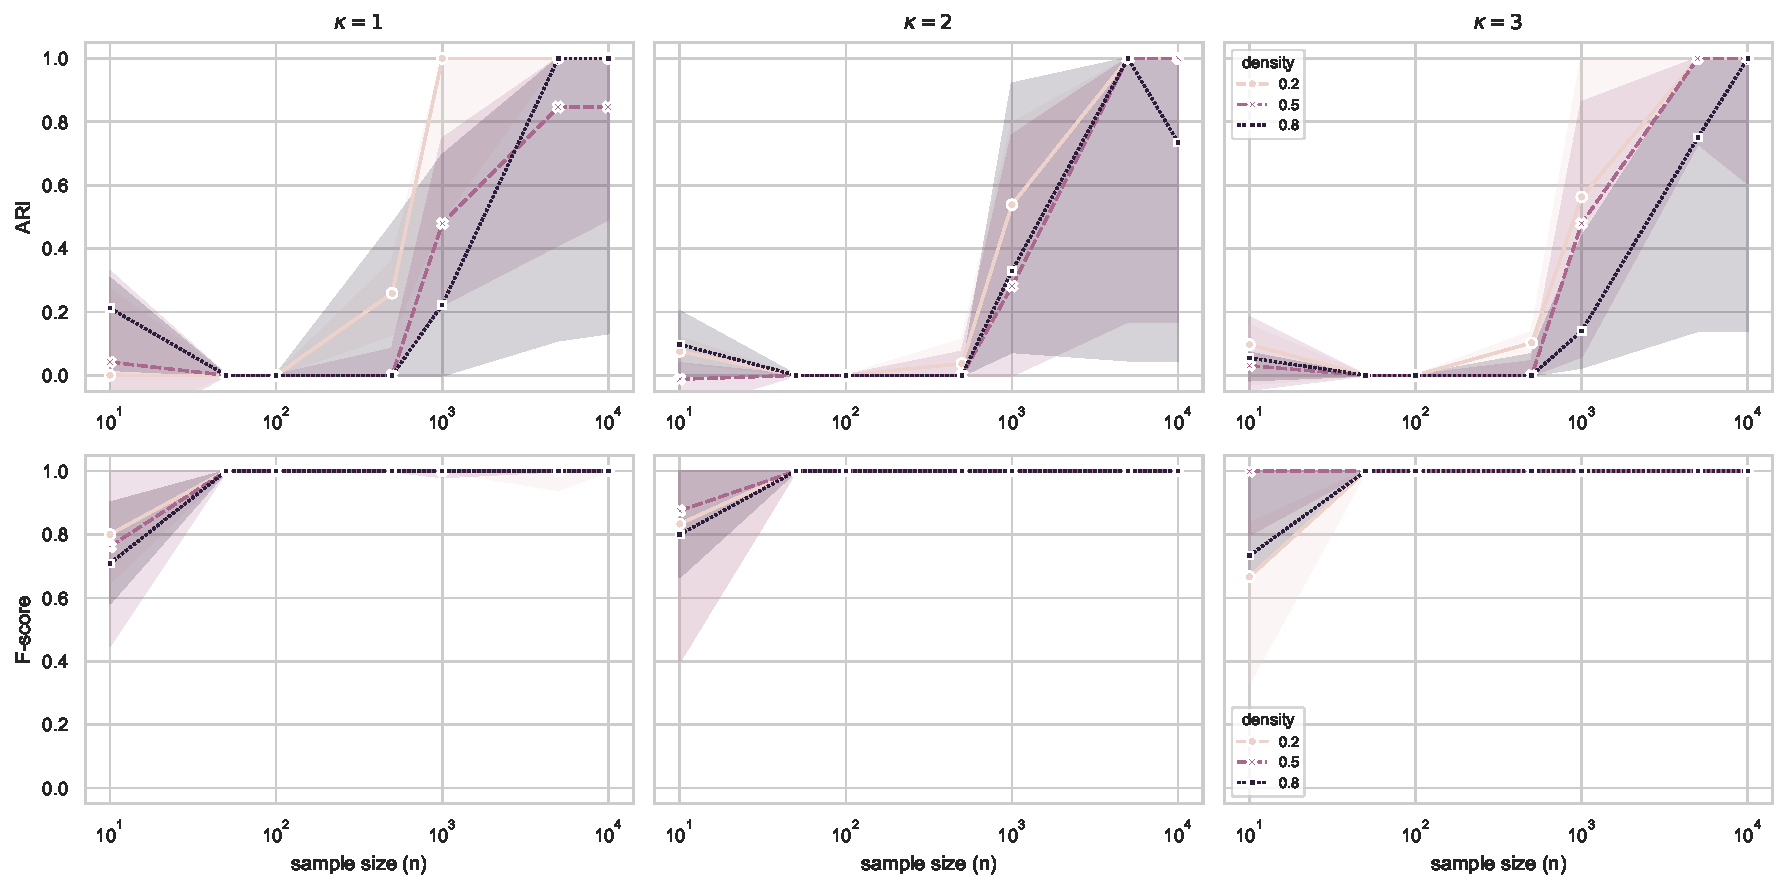
\includegraphics[width=\textwidth]{figures/synth_main.pdf}
    \caption{Synthetic-data evaluation of the \texttt{Lacerda} recipe, three seeds per cell, as the sample size $n$ varies. Columns index the number of cycles $\kappa$. \textbf{Top:} ARI between predicted and true SCC partition. \textbf{Middle:} inter-SCC $F_1$ (variable-level edges restricted to pairs in different true SCCs) — converges to 1, illustrating Theorem~\ref{thm:condensation-id}. \textbf{Bottom:} variable-level $F_1$ on the full DAG — saturates below 1; the gap is the unidentifiable intra-SCC structure.}
    \label{fig:results}
\end{figure}


% =============================================================================
\section{Discussion}
\label{sec:discussion}
% =============================================================================

We have shown that the coarsening framework of \citet{madaleno2025coarsening} extends naturally to directed graphs with cycles, with the SCC partition as the lattice floor and the condensation DAG as the canonical identification target. The central theorem (Theorem~\ref{thm:condensation-id}) sharpens the cyclic-SEM identifiability picture of \citet{lacerda2008discovering}: although the underlying micro-graph is identifiable only up to a distributional equivalence class, its condensation is fully identifiable from the observational distribution. This identification result is what licenses applying C-DAG causal-effect identification \citep{anand2023causal} to the recovered structure.

The observational approach requires linear non-Gaussian noise and no latent confounders --- a stronger assumption than the Gaussianity sufficient for the intervention-determined approach, but with the substantial practical advantage of needing no interventions at all. Hard (do) interventions on a single variable, which sever the cyclic mechanism, are excluded throughout; only soft (shift) interventions and hard interventions on entire SCCs are well-defined in the cyclic SEM setting (\S\ref{sec:effects}).

\paragraph{Open directions.} (i) Latent-confounder generalisations via overcomplete ICA \citep{salehkaleybar2020learning,dai2026distributional}: the path-rank identity and Theorem~\ref{thm:scc-tc} carry over because they are independent of the source/observed dimension. (ii) Mixed-Gaussian extension --- the path-rank argument survives intra-SCC Gaussian noise as long as at most one source per SCC is Gaussian, which would address \citet[\S6]{lacerda2008discovering}'s open problem on Gaussian/non-Gaussian mixtures. (iii) An empirical realisation of cluster-level causal-effect estimation on the recovered C-DAG, beyond the theoretical bridge sketched in \S\ref{sec:effects}. (iv) Characterising the cyclic-coarsening lattice (the broader generalisation noted in \S\ref{sec:scc-floor}) and identifying which of its elements are recoverable from data.


% =============================================================================
% References
% =============================================================================
\bibliographystyle{plainnat}

\begin{thebibliography}{10}

\bibitem[Madaleno et~al.(2025)]{madaleno2025coarsening}
Francisco Madaleno, Pratik Misra, and Alex Markham.
\newblock Coarsening causal {DAG} models.
\newblock \emph{arXiv preprint arXiv:2601.10531}, 2025.

\bibitem[Dai et~al.(2026)]{dai2026distributional}
Haoyue Dai, Immanuel Albrecht, Peter Spirtes, and Kun Zhang.
\newblock Distributional equivalence in linear non-{G}aussian latent-variable cyclic causal models: Characterization and learning.
\newblock In \emph{International Conference on Learning Representations (ICLR)}, 2026.

\bibitem[Eriksson \& Koivunen(2004)]{eriksson2004identifiability}
Jan Eriksson and Visa Koivunen.
\newblock Identifiability, separability, and uniqueness of linear {ICA} models.
\newblock \emph{IEEE Signal Processing Letters}, 11(7):601--604, 2004.

\bibitem[Salehkaleybar et~al.(2020)]{salehkaleybar2020learning}
Saber Salehkaleybar, Amiremad Ghassami, Negar Kiyavash, and Kun Zhang.
\newblock Learning linear non-{G}aussian causal models in the presence of latent variables.
\newblock \emph{Journal of Machine Learning Research}, 21(39):1--24, 2020.

\bibitem[Lacerda et~al.(2008)]{lacerda2008discovering}
Gustavo Lacerda, Peter Spirtes, Joseph Ramsey, and Patrik~O. Hoyer.
\newblock Discovering cyclic causal models by independent components analysis.
\newblock In \emph{Conference on Uncertainty in Artificial Intelligence (UAI)}, 2008.

\bibitem[Tarjan(1972)]{tarjan1972depth}
Robert Tarjan.
\newblock Depth-first search and linear graph algorithms.
\newblock \emph{SIAM Journal on Computing}, 1(2):146--160, 1972.

\bibitem[Spirtes(1995)]{spirtes1995directed}
Peter Spirtes.
\newblock Directed cyclic graphical representations of feedback models.
\newblock In \emph{Conference on Uncertainty in Artificial Intelligence (UAI)}, 1995.

\bibitem[Bongers et~al.(2021)]{bongers2021foundations}
Stephan Bongers, Patrick Forr{\'e}, Jonas Peters, and Joris~M. Mooij.
\newblock Foundations of structural causal models with cycles and latent variables.
\newblock \emph{Annals of Statistics}, 49(5):2885--2915, 2021.

\bibitem[Hyv{\"a}rinen(1999)]{hyvarinen1999fast}
Aapo Hyv{\"a}rinen.
\newblock Fast and robust fixed-point algorithms for independent component analysis.
\newblock \emph{IEEE Transactions on Neural Networks}, 10(3):626--634, 1999.

\bibitem[Kuhn(1955)]{kuhn1955hungarian}
Harold~W. Kuhn.
\newblock The {Hungarian} method for the assignment problem.
\newblock \emph{Naval Research Logistics Quarterly}, 2(1--2):83--97, 1955.

\bibitem[Gretton et~al.(2008)]{gretton2008kernel}
Arthur Gretton, Kenji Fukumizu, Choon~H. Teo, Le Song, Bernhard Sch{\"o}lkopf, and Alex~J. Smola.
\newblock A kernel statistical test of independence.
\newblock In \emph{Advances in Neural Information Processing Systems (NeurIPS)}, 2008.

\bibitem[Maeda \& Shimizu(2020)]{maeda2020rcd}
Takashi~N. Maeda and Shohei Shimizu.
\newblock {RCD}: Repetitive causal discovery of linear non-{G}aussian acyclic models with latent confounders.
\newblock In \emph{International Conference on Artificial Intelligence and Statistics (AISTATS)}, 2020.

\bibitem[Lewicki \& Sejnowski(2000)]{lewicki2000learning}
Michael~S. Lewicki and Terrence~J. Sejnowski.
\newblock Learning overcomplete representations.
\newblock \emph{Neural Computation}, 12(2):337--365, 2000.

\bibitem[Forr{\'e} \& Mooij(2018)]{forre2018constraint}
Patrick Forr{\'e} and Joris~M. Mooij.
\newblock Constraint-based causal discovery for non-linear structural causal models with cycles and latent confounders.
\newblock In \emph{Conference on Uncertainty in Artificial Intelligence (UAI)}, 2018.

\bibitem[Gabow(2000)]{gabow2000path}
Harold~N. Gabow.
\newblock Path-based depth-first search for strong and biconnected components.
\newblock \emph{Information Processing Letters}, 74(3--4):107--114, 2000.

\bibitem[Rubenstein et~al.(2017)]{rubenstein2017causal}
Paul~K. Rubenstein, Sebastian Weichwald, Stephan Bongers, Joris~M. Mooij, Dominik Janzing, Moritz Grosse-Wentrup, and Bernhard Sch{\"o}lkopf.
\newblock Causal consistency of structural equation models.
\newblock In \emph{Conference on Uncertainty in Artificial Intelligence (UAI)}, 2017.

\bibitem[Beckers \& Halpern(2019)]{beckers2020approximate}
Sander Beckers and Joseph~Y. Halpern.
\newblock Abstracting causal models.
\newblock In \emph{AAAI Conference on Artificial Intelligence}, 2019.

\bibitem[Wahl et~al.(2025)]{wahl2025foundations}
Jonas Wahl, Sofia Faltenbacher, and Jakob Runge.
\newblock Foundations of group-level causal discovery.
\newblock 2025.

\bibitem[Petersen et~al.(2025)]{petersen2025structural}
Anne~H. Petersen et al.
\newblock Structural baseline coarsening of causal {DAG}s.
\newblock In \emph{Causal Learning and Reasoning (CLeaR)}, 2025.

\bibitem[Anand et~al.(2023)]{anand2023causal}
Tara~V. Anand, Ad{\`e}le~H. Ribeiro, Jin Tian, and Elias Bareinboim.
\newblock Causal effect identification in cluster {DAG}s.
\newblock In \emph{AAAI Conference on Artificial Intelligence}, 2023.

\end{thebibliography}


% =============================================================================
\appendix
\section{Proofs}
\label{app:proofs}
% =============================================================================

For a directed graph $G = (V, E)$, denote the existence of a directed path from vertex $u$ to vertex $v$ by the reachability relation $u \leadsto_G v$. By convention, a vertex can always reach itself (paths of length 0), so $u \leadsto_G u$ for all $u \in V$.

\begin{definition}[Strongly connected component]
\label{def:scc}
Define a binary relation $\sim_G$ on $V$ by
\[
u \sim_G v \iff (u \leadsto_G v) \land (v \leadsto_G u).
\]
The relation $\sim_G$ is an equivalence relation (reflexive, symmetric, transitive). A \emph{strongly connected component} (SCC) of $G$ is an equivalence class of $V$ under $\sim_G$.
\end{definition}

\begin{definition}[Transitive closure]
\label{def:transitive-closure}
The \emph{transitive closure} of a directed graph $G = (V, E)$ is the graph $G^* = (V, E^*)$ with edge set
\[
E^* = \{ (u, v) \in V \times V \mid u \leadsto_G v \}.
\]
\end{definition}

\begin{theorem}[SCCs are preserved under transitive closure]
\label{thm:scc-tc}
Let $G = (V, E)$ be a directed graph and let $G^* = (V, E^*)$ be its transitive closure. Then $G$ and $G^*$ have the same SCCs.
\end{theorem}

\begin{proof}
It suffices to show $u \sim_G v \iff u \sim_{G^*} v$ for all $u, v \in V$.

\noindent($\Rightarrow$) Suppose $u \sim_G v$, so $u \leadsto_G v$ and $v \leadsto_G u$. By Definition~\ref{def:transitive-closure}, $(u, v) \in E^*$ and $(v, u) \in E^*$, hence $u \leadsto_{G^*} v$ and $v \leadsto_{G^*} u$, i.e.\ $u \sim_{G^*} v$.

\noindent($\Leftarrow$) Suppose $u \sim_{G^*} v$, so there is a path $u = x_0, x_1, \dots, x_k = v$ in $G^*$. Each step $(x_i, x_{i+1}) \in E^*$ implies $x_i \leadsto_G x_{i+1}$ by Definition~\ref{def:transitive-closure}. Transitivity of $\leadsto_G$ then gives $u \leadsto_G v$. Symmetric reasoning yields $v \leadsto_G u$, so $u \sim_G v$.

The two implications give equality of equivalence classes, hence equality of SCCs.
\end{proof}

Theorem~\ref{thm:scc-tc} is the structural fact underlying Approach~2 (\S\ref{sec:approach-oica}): even though plain ICA recovers $\mathrm{supp}(A)$ — the adjacency of the transitive closure of $G$ rather than of $G$ itself — the SCC partition we extract from it is exactly the SCC partition of $G$.

\end{document}
